\documentclass[1p]{elsarticle_modified}
%\bibliographystyle{elsarticle-num}

%\usepackage[colorlinks]{hyperref}
%\usepackage{abbrmath_seonhwa} %\Abb, \Ascr, \Acal ,\Abf, \Afrak
\usepackage{amsfonts}
\usepackage{amssymb}
\usepackage{amsmath}
\usepackage{amsthm}
\usepackage{scalefnt}
\usepackage{amsbsy}
\usepackage{kotex}
\usepackage{caption}
\usepackage{subfig}
\usepackage{color}
\usepackage{graphicx}
\usepackage{xcolor} %% white, black, red, green, blue, cyan, magenta, yellow
\usepackage{float}
\usepackage{setspace}
\usepackage{hyperref}

\usepackage{tikz}
\usetikzlibrary{arrows}

\usepackage{multirow}
\usepackage{array} % fixed length table
\usepackage{hhline}

%%%%%%%%%%%%%%%%%%%%%
\makeatletter
\renewcommand*\env@matrix[1][\arraystretch]{%
	\edef\arraystretch{#1}%
	\hskip -\arraycolsep
	\let\@ifnextchar\new@ifnextchar
	\array{*\c@MaxMatrixCols c}}
\makeatother %https://tex.stackexchange.com/questions/14071/how-can-i-increase-the-line-spacing-in-a-matrix
%%%%%%%%%%%%%%%

\usepackage[normalem]{ulem}

\newcommand{\msout}[1]{\ifmmode\text{\sout{\ensuremath{#1}}}\else\sout{#1}\fi}
%SOURCE: \msout is \stkout macro in https://tex.stackexchange.com/questions/20609/strikeout-in-math-mode

\newcommand{\cancel}[1]{
	\ifmmode
	{\color{red}\msout{#1}}
	\else
	{\color{red}\sout{#1}}
	\fi
}

\newcommand{\add}[1]{
	{\color{blue}\uwave{#1}}
}

\newcommand{\replace}[2]{
	\ifmmode
	{\color{red}\msout{#1}}{\color{blue}\uwave{#2}}
	\else
	{\color{red}\sout{#1}}{\color{blue}\uwave{#2}}
	\fi
}

\newcommand{\Sol}{\mathcal{S}} %segment
\newcommand{\D}{D} %diagram
\newcommand{\A}{\mathcal{A}} %arc


%%%%%%%%%%%%%%%%%%%%%%%%%%%%%5 test

\def\sl{\operatorname{\textup{SL}}(2,\Cbb)}
\def\psl{\operatorname{\textup{PSL}}(2,\Cbb)}
\def\quan{\mkern 1mu \triangleright \mkern 1mu}

\theoremstyle{definition}
\newtheorem{thm}{Theorem}[section]
\newtheorem{prop}[thm]{Proposition}
\newtheorem{lem}[thm]{Lemma}
\newtheorem{ques}[thm]{Question}
\newtheorem{cor}[thm]{Corollary}
\newtheorem{defn}[thm]{Definition}
\newtheorem{exam}[thm]{Example}
\newtheorem{rmk}[thm]{Remark}
\newtheorem{alg}[thm]{Algorithm}

\newcommand{\I}{\sqrt{-1}}
\begin{document}

%\begin{frontmatter}
%
%\title{Boundary parabolic representations of knots up to 8 crossings}
%
%%% Group authors per affiliation:
%\author{Yunhi Cho} 
%\address{Department of Mathematics, University of Seoul, Seoul, Korea}
%\ead{yhcho@uos.ac.kr}
%
%
%\author{Seonhwa Kim} %\fnref{s_kim}}
%\address{Center for Geometry and Physics, Institute for Basic Science, Pohang, 37673, Korea}
%\ead{ryeona17@ibs.re.kr}
%
%\author{Hyuk Kim}
%\address{Department of Mathematical Sciences, Seoul National University, Seoul 08826, Korea}
%\ead{hyukkim@snu.ac.kr}
%
%\author{Seokbeom Yoon}
%\address{Department of Mathematical Sciences, Seoul National University, Seoul, 08826,  Korea}
%\ead{sbyoon15@snu.ac.kr}
%
%\begin{abstract}
%We find all boundary parabolic representation of knots up to 8 crossings.
%
%\end{abstract}
%\begin{keyword}
%    \MSC[2010] 57M25 
%\end{keyword}
%
%\end{frontmatter}

%\linenumbers
%\tableofcontents
%
\newcommand\colored[1]{\textcolor{white}{\rule[-0.35ex]{0.8em}{1.4ex}}\kern-0.8em\color{red} #1}%
%\newcommand\colored[1]{\textcolor{white}{ #1}\kern-2.17ex	\textcolor{white}{ #1}\kern-1.81ex	\textcolor{white}{ #1}\kern-2.15ex\color{red}#1	}

{\Large $\underline{12a_{0933}~(K12a_{0933})}$}

\setlength{\tabcolsep}{10pt}
\renewcommand{\arraystretch}{1.6}
\vspace{1cm}\begin{tabular}{m{100pt}>{\centering\arraybackslash}m{274pt}}
\multirow{5}{120pt}{
	\centering
	\includegraphics[width=112pt]{../../../GIT/diagram.site/Diagrams/png/1734_12a_0933.png}\\
\ \ \ A knot diagram\footnotemark}&
\allowdisplaybreaks
\textbf{Linearized knot diagam} \\
\cline{2-2}
 &
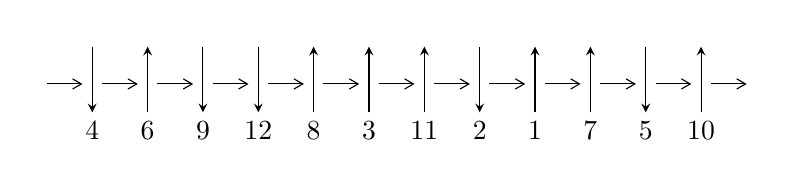
\begin{tikzpicture}[x=20pt, y=17pt]
	% nodes
	\node (C0) at (0, 0) {};
	\node (C1) at (1, 0) {};
	\node (C1U) at (1, +1) {};
	\node (C1D) at (1, -1) {4};

	\node (C2) at (2, 0) {};
	\node (C2U) at (2, +1) {};
	\node (C2D) at (2, -1) {6};

	\node (C3) at (3, 0) {};
	\node (C3U) at (3, +1) {};
	\node (C3D) at (3, -1) {9};

	\node (C4) at (4, 0) {};
	\node (C4U) at (4, +1) {};
	\node (C4D) at (4, -1) {12};

	\node (C5) at (5, 0) {};
	\node (C5U) at (5, +1) {};
	\node (C5D) at (5, -1) {8};

	\node (C6) at (6, 0) {};
	\node (C6U) at (6, +1) {};
	\node (C6D) at (6, -1) {3};

	\node (C7) at (7, 0) {};
	\node (C7U) at (7, +1) {};
	\node (C7D) at (7, -1) {11};

	\node (C8) at (8, 0) {};
	\node (C8U) at (8, +1) {};
	\node (C8D) at (8, -1) {2};

	\node (C9) at (9, 0) {};
	\node (C9U) at (9, +1) {};
	\node (C9D) at (9, -1) {1};

	\node (C10) at (10, 0) {};
	\node (C10U) at (10, +1) {};
	\node (C10D) at (10, -1) {7};

	\node (C11) at (11, 0) {};
	\node (C11U) at (11, +1) {};
	\node (C11D) at (11, -1) {5};

	\node (C12) at (12, 0) {};
	\node (C12U) at (12, +1) {};
	\node (C12D) at (12, -1) {10};
	\node (C13) at (13, 0) {};

	% arrows
	\draw[->,>={angle 60}]
	(C0) edge (C1) (C1) edge (C2) (C2) edge (C3) (C3) edge (C4) (C4) edge (C5) (C5) edge (C6) (C6) edge (C7) (C7) edge (C8) (C8) edge (C9) (C9) edge (C10) (C10) edge (C11) (C11) edge (C12) (C12) edge (C13) ;	\draw[->,>=stealth]
	(C1U) edge (C1D) (C2D) edge (C2U) (C3U) edge (C3D) (C4U) edge (C4D) (C5D) edge (C5U) (C6D) edge (C6U) (C7D) edge (C7U) (C8U) edge (C8D) (C9D) edge (C9U) (C10D) edge (C10U) (C11U) edge (C11D) (C12D) edge (C12U) ;
	\end{tikzpicture} \\
\hhline{~~} \\& 
\textbf{Solving Sequence} \\ \cline{2-2} 
 &
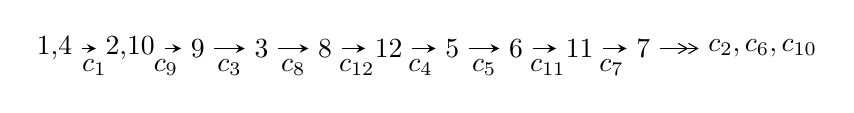
\begin{tikzpicture}[x=23pt, y=7pt]
	% node
	\node (A0) at (-1/8, 0) {1,4};
	\node (A1) at (17/16, 0) {2,10};
	\node (A2) at (17/8, 0) {9};
	\node (A3) at (25/8, 0) {3};
	\node (A4) at (33/8, 0) {8};
	\node (A5) at (41/8, 0) {12};
	\node (A6) at (49/8, 0) {5};
	\node (A7) at (57/8, 0) {6};
	\node (A8) at (65/8, 0) {11};
	\node (A9) at (73/8, 0) {7};
	\node (C1) at (1/2, -1) {$c_{1}$};
	\node (C2) at (13/8, -1) {$c_{9}$};
	\node (C3) at (21/8, -1) {$c_{3}$};
	\node (C4) at (29/8, -1) {$c_{8}$};
	\node (C5) at (37/8, -1) {$c_{12}$};
	\node (C6) at (45/8, -1) {$c_{4}$};
	\node (C7) at (53/8, -1) {$c_{5}$};
	\node (C8) at (61/8, -1) {$c_{11}$};
	\node (C9) at (69/8, -1) {$c_{7}$};
	\node (A10) at (11, 0) {$c_{2},c_{6},c_{10}$};

	% edge
	\draw[->,>=stealth]	
	(A0) edge (A1) (A1) edge (A2) (A2) edge (A3) (A3) edge (A4) (A4) edge (A5) (A5) edge (A6) (A6) edge (A7) (A7) edge (A8) (A8) edge (A9) ;
	\draw[->>,>={angle 60}]	
	(A9) edge (A10);
\end{tikzpicture} \\ 

\end{tabular} \\

\footnotetext{
The image of knot diagram is generated by the software ``\textbf{Draw programme}" developed by Andrew Bartholomew(\url{http://www.layer8.co.uk/maths/draw/index.htm\#Running-draw}), where we modified some parts for our purpose(\url{https://github.com/CATsTAILs/LinksPainter}).
}\phantom \\ \newline 
\centering \textbf{Ideals for irreducible components\footnotemark of $X_{\text{par}}$} 
 
\begin{align*}
I^u_{1}&=\langle 
7.45874\times10^{1495} u^{151}+1.33532\times10^{1497} u^{150}+\cdots+3.64559\times10^{1494} b+4.30408\times10^{1496},\\
\phantom{I^u_{1}}&\phantom{= \langle  }-5.52856\times10^{1496} u^{151}-9.82856\times10^{1497} u^{150}+\cdots+3.64559\times10^{1494} a-1.60537\times10^{1497},\\
\phantom{I^u_{1}}&\phantom{= \langle  }u^{152}+18 u^{151}+\cdots+39 u+1\rangle \\
I^u_{2}&=\langle 
2.35650\times10^{100} u^{38}-3.38206\times10^{100} u^{37}+\cdots+3.27749\times10^{101} b+1.72182\times10^{102},\\
\phantom{I^u_{2}}&\phantom{= \langle  }9.76286\times10^{101} u^{38}-8.69104\times10^{101} u^{37}+\cdots+3.27749\times10^{101} a+9.71584\times10^{102},\;u^{39}- u^{38}+\cdots+28 u-1\rangle \\
\\
\end{align*}
\raggedright * 2 irreducible components of $\dim_{\mathbb{C}}=0$, with total 191 representations.\\
\footnotetext{All coefficients of polynomials are rational numbers. But the coefficients are sometimes approximated in decimal forms when there is not enough margin.}
\newpage
\renewcommand{\arraystretch}{1}
\centering \section*{I. $I^u_{1}= \langle 7.46\times10^{1495} u^{151}+1.34\times10^{1497} u^{150}+\cdots+3.65\times10^{1494} b+4.30\times10^{1496},\;-5.53\times10^{1496} u^{151}-9.83\times10^{1497} u^{150}+\cdots+3.65\times10^{1494} a-1.61\times10^{1497},\;u^{152}+18 u^{151}+\cdots+39 u+1 \rangle$}
\flushleft \textbf{(i) Arc colorings}\\
\begin{tabular}{m{7pt} m{180pt} m{7pt} m{180pt} }
\flushright $a_{1}=$&$\begin{pmatrix}1\\0\end{pmatrix}$ \\
\flushright $a_{4}=$&$\begin{pmatrix}0\\u\end{pmatrix}$ \\
\flushright $a_{2}=$&$\begin{pmatrix}1\\u^2\end{pmatrix}$ \\
\flushright $a_{10}=$&$\begin{pmatrix}151.651 u^{151}+2696.01 u^{150}+\cdots+17353.5 u+440.358\\-20.4596 u^{151}-366.282 u^{150}+\cdots-4076.80 u-118.063\end{pmatrix}$ \\
\flushright $a_{9}=$&$\begin{pmatrix}172.110 u^{151}+3062.29 u^{150}+\cdots+21430.3 u+558.421\\-20.4596 u^{151}-366.282 u^{150}+\cdots-4076.80 u-118.063\end{pmatrix}$ \\
\flushright $a_{3}=$&$\begin{pmatrix}319.100 u^{151}+5726.02 u^{150}+\cdots+85918.0 u+2583.86\\-11.0235 u^{151}-194.799 u^{150}+\cdots-924.820 u-30.9225\end{pmatrix}$ \\
\flushright $a_{8}=$&$\begin{pmatrix}146.852 u^{151}+2609.75 u^{150}+\cdots+16133.8 u+404.669\\-19.8946 u^{151}-356.472 u^{150}+\cdots-4133.32 u-120.159\end{pmatrix}$ \\
\flushright $a_{12}=$&$\begin{pmatrix}-3.32451 u^{151}-57.0384 u^{150}+\cdots+6814.87 u+268.841\\-34.2470 u^{151}-602.620 u^{150}+\cdots-849.480 u-12.3166\end{pmatrix}$ \\
\flushright $a_{5}=$&$\begin{pmatrix}157.788 u^{151}+2843.03 u^{150}+\cdots+54408.2 u+1659.71\\36.0042 u^{151}+647.930 u^{150}+\cdots+7325.33 u+201.311\end{pmatrix}$ \\
\flushright $a_{6}=$&$\begin{pmatrix}60.6871 u^{151}+1097.66 u^{150}+\cdots+31667.6 u+1035.03\\-2.47249 u^{151}-46.0628 u^{150}+\cdots-1190.55 u-36.7659\end{pmatrix}$ \\
\flushright $a_{11}=$&$\begin{pmatrix}679.004 u^{151}+12120.8 u^{150}+\cdots+112833. u+3113.90\\25.1544 u^{151}+447.720 u^{150}+\cdots+877.076 u-0.217198\end{pmatrix}$ \\
\flushright $a_{7}=$&$\begin{pmatrix}-676.104 u^{151}-12070.4 u^{150}+\cdots-113192. u-3126.36\\-10.1138 u^{151}-181.931 u^{150}+\cdots-69.6124 u+18.2014\end{pmatrix}$\\&\end{tabular}
\flushleft \textbf{(ii) Obstruction class $= -1$}\\~\\
\flushleft \textbf{(iii) Cusp Shapes $= 320.886 u^{151}+5727.00 u^{150}+\cdots+47503.8 u+1336.04$}\\~\\
\newpage\renewcommand{\arraystretch}{1}
\flushleft \textbf{(iv) u-Polynomials at the component}\newline \\
\begin{tabular}{m{50pt}|m{274pt}}
Crossings & \hspace{64pt}u-Polynomials at each crossing \\
\hline $$\begin{aligned}c_{1}\end{aligned}$$&$\begin{aligned}
&u^{152}-18 u^{151}+\cdots-39 u+1
\end{aligned}$\\
\hline $$\begin{aligned}c_{2},c_{6}\end{aligned}$$&$\begin{aligned}
&u^{152}-3 u^{151}+\cdots+225401 u-8611
\end{aligned}$\\
\hline $$\begin{aligned}c_{3}\end{aligned}$$&$\begin{aligned}
&u^{152}- u^{151}+\cdots-15926 u-2857
\end{aligned}$\\
\hline $$\begin{aligned}c_{4},c_{11}\end{aligned}$$&$\begin{aligned}
&u^{152}+2 u^{151}+\cdots-7903029 u+617167
\end{aligned}$\\
\hline $$\begin{aligned}c_{5}\end{aligned}$$&$\begin{aligned}
&u^{152}+5 u^{151}+\cdots+305455361572 u+24617683931
\end{aligned}$\\
\hline $$\begin{aligned}c_{7},c_{10}\end{aligned}$$&$\begin{aligned}
&u^{152}+6 u^{151}+\cdots-4623182 u+1967081
\end{aligned}$\\
\hline $$\begin{aligned}c_{8}\end{aligned}$$&$\begin{aligned}
&u^{152}+3 u^{151}+\cdots+438574749 u-20742433
\end{aligned}$\\
\hline $$\begin{aligned}c_{9},c_{12}\end{aligned}$$&$\begin{aligned}
&u^{152}+9 u^{151}+\cdots-369447 u+44911
\end{aligned}$\\
\hline
\end{tabular}\\~\\
\newpage\renewcommand{\arraystretch}{1}
\flushleft \textbf{(v) Riley Polynomials at the component}\newline \\
\begin{tabular}{m{50pt}|m{274pt}}
Crossings & \hspace{64pt}Riley Polynomials at each crossing \\
\hline $$\begin{aligned}c_{1}\end{aligned}$$&$\begin{aligned}
&y^{152}+56 y^{151}+\cdots+23 y+1
\end{aligned}$\\
\hline $$\begin{aligned}c_{2},c_{6}\end{aligned}$$&$\begin{aligned}
&y^{152}-101 y^{151}+\cdots-16415773991 y+74149321
\end{aligned}$\\
\hline $$\begin{aligned}c_{3}\end{aligned}$$&$\begin{aligned}
&y^{152}-39 y^{151}+\cdots-753263922 y+8162449
\end{aligned}$\\
\hline $$\begin{aligned}c_{4},c_{11}\end{aligned}$$&$\begin{aligned}
&y^{152}+124 y^{151}+\cdots-8121102240761 y+380895105889
\end{aligned}$\\
\hline $$\begin{aligned}c_{5}\end{aligned}$$&$\begin{aligned}
&y^{152}-63 y^{151}+\cdots-2.20\times10^{22} y+6.06\times10^{20}
\end{aligned}$\\
\hline $$\begin{aligned}c_{7},c_{10}\end{aligned}$$&$\begin{aligned}
&y^{152}-96 y^{151}+\cdots-110104889750638 y+3869407660561
\end{aligned}$\\
\hline $$\begin{aligned}c_{8}\end{aligned}$$&$\begin{aligned}
&y^{152}+29 y^{151}+\cdots+22531234880768715 y+430248526759489
\end{aligned}$\\
\hline $$\begin{aligned}c_{9},c_{12}\end{aligned}$$&$\begin{aligned}
&y^{152}+79 y^{151}+\cdots-258835027171 y+2016997921
\end{aligned}$\\
\hline
\end{tabular}\\~\\
\newpage\flushleft \textbf{(vi) Complex Volumes and Cusp Shapes}
$$\begin{array}{c|c|c}  
\text{Solutions to }I^u_{1}& \I (\text{vol} + \sqrt{-1}CS) & \text{Cusp shape}\\
 \hline 
\begin{aligned}
u &= -0.935275 + 0.382584 I \\
a &= \phantom{-}0.08390 + 1.52785 I \\
b &= \phantom{-}0.65486 + 1.28889 I\end{aligned}
 & \phantom{-}1.99484 + 7.85089 I & \phantom{-0.000000 } 0 \\ \hline\begin{aligned}
u &= -0.935275 - 0.382584 I \\
a &= \phantom{-}0.08390 - 1.52785 I \\
b &= \phantom{-}0.65486 - 1.28889 I\end{aligned}
 & \phantom{-}1.99484 - 7.85089 I & \phantom{-0.000000 } 0 \\ \hline\begin{aligned}
u &= -0.233837 + 0.951544 I \\
a &= \phantom{-}0.84492 + 1.22874 I \\
b &= \phantom{-}0.011769 - 0.796786 I\end{aligned}
 & \phantom{-}5.20569 + 4.08312 I & \phantom{-0.000000 } 0 \\ \hline\begin{aligned}
u &= -0.233837 - 0.951544 I \\
a &= \phantom{-}0.84492 - 1.22874 I \\
b &= \phantom{-}0.011769 + 0.796786 I\end{aligned}
 & \phantom{-}5.20569 - 4.08312 I & \phantom{-0.000000 } 0 \\ \hline\begin{aligned}
u &= -0.281681 + 0.898653 I \\
a &= -1.43264 - 1.13703 I \\
b &= \phantom{-}0.171388 + 1.015400 I\end{aligned}
 & \phantom{-}6.18918 + 3.73765 I & \phantom{-0.000000 } 0 \\ \hline\begin{aligned}
u &= -0.281681 - 0.898653 I \\
a &= -1.43264 + 1.13703 I \\
b &= \phantom{-}0.171388 - 1.015400 I\end{aligned}
 & \phantom{-}6.18918 - 3.73765 I & \phantom{-0.000000 } 0 \\ \hline\begin{aligned}
u &= -0.679834 + 0.648725 I \\
a &= \phantom{-}0.204352 - 0.815495 I \\
b &= -0.553882 + 0.286722 I\end{aligned}
 & \phantom{-}6.54096 - 3.13281 I & \phantom{-0.000000 } 0 \\ \hline\begin{aligned}
u &= -0.679834 - 0.648725 I \\
a &= \phantom{-}0.204352 + 0.815495 I \\
b &= -0.553882 - 0.286722 I\end{aligned}
 & \phantom{-}6.54096 + 3.13281 I & \phantom{-0.000000 } 0 \\ \hline\begin{aligned}
u &= -0.916063 + 0.201408 I \\
a &= -0.470095 + 1.330040 I \\
b &= \phantom{-}0.141253 + 1.252060 I\end{aligned}
 & -3.67199 - 2.16904 I & \phantom{-0.000000 } 0 \\ \hline\begin{aligned}
u &= -0.916063 - 0.201408 I \\
a &= -0.470095 - 1.330040 I \\
b &= \phantom{-}0.141253 - 1.252060 I\end{aligned}
 & -3.67199 + 2.16904 I & \phantom{-0.000000 } 0\\
 \hline 
 \end{array}$$\newpage$$\begin{array}{c|c|c}  
\text{Solutions to }I^u_{1}& \I (\text{vol} + \sqrt{-1}CS) & \text{Cusp shape}\\
 \hline 
\begin{aligned}
u &= \phantom{-}0.370334 + 0.995863 I \\
a &= -0.073221 - 0.365053 I \\
b &= -0.948877 + 0.133965 I\end{aligned}
 & \phantom{-}3.19199 - 2.62186 I & \phantom{-0.000000 } 0 \\ \hline\begin{aligned}
u &= \phantom{-}0.370334 - 0.995863 I \\
a &= -0.073221 + 0.365053 I \\
b &= -0.948877 - 0.133965 I\end{aligned}
 & \phantom{-}3.19199 + 2.62186 I & \phantom{-0.000000 } 0 \\ \hline\begin{aligned}
u &= \phantom{-}0.160558 + 1.079900 I \\
a &= \phantom{-}0.185601 + 0.556425 I \\
b &= \phantom{-}0.766670 - 0.185969 I\end{aligned}
 & \phantom{-}6.41663 + 2.23215 I & \phantom{-0.000000 } 0 \\ \hline\begin{aligned}
u &= \phantom{-}0.160558 - 1.079900 I \\
a &= \phantom{-}0.185601 - 0.556425 I \\
b &= \phantom{-}0.766670 + 0.185969 I\end{aligned}
 & \phantom{-}6.41663 - 2.23215 I & \phantom{-0.000000 } 0 \\ \hline\begin{aligned}
u &= -0.721807 + 0.549581 I \\
a &= -0.489303 - 0.074539 I \\
b &= \phantom{-}0.659359 - 0.257865 I\end{aligned}
 & \phantom{-}1.42163 + 4.80254 I & \phantom{-0.000000 } 0 \\ \hline\begin{aligned}
u &= -0.721807 - 0.549581 I \\
a &= -0.489303 + 0.074539 I \\
b &= \phantom{-}0.659359 + 0.257865 I\end{aligned}
 & \phantom{-}1.42163 - 4.80254 I & \phantom{-0.000000 } 0 \\ \hline\begin{aligned}
u &= \phantom{-}0.811230 + 0.754642 I \\
a &= \phantom{-}0.466320 + 0.975953 I \\
b &= -0.52368 + 1.41851 I\end{aligned}
 & -1.90553 - 6.31711 I & \phantom{-0.000000 } 0 \\ \hline\begin{aligned}
u &= \phantom{-}0.811230 - 0.754642 I \\
a &= \phantom{-}0.466320 - 0.975953 I \\
b &= -0.52368 - 1.41851 I\end{aligned}
 & -1.90553 + 6.31711 I & \phantom{-0.000000 } 0 \\ \hline\begin{aligned}
u &= \phantom{-}1.058100 + 0.348509 I \\
a &= -0.608381 - 0.934220 I \\
b &= \phantom{-}0.341759 - 1.058760 I\end{aligned}
 & -3.68720 - 1.29648 I & \phantom{-0.000000 } 0 \\ \hline\begin{aligned}
u &= \phantom{-}1.058100 - 0.348509 I \\
a &= -0.608381 + 0.934220 I \\
b &= \phantom{-}0.341759 + 1.058760 I\end{aligned}
 & -3.68720 + 1.29648 I & \phantom{-0.000000 } 0\\
 \hline 
 \end{array}$$\newpage$$\begin{array}{c|c|c}  
\text{Solutions to }I^u_{1}& \I (\text{vol} + \sqrt{-1}CS) & \text{Cusp shape}\\
 \hline 
\begin{aligned}
u &= -0.644387 + 0.911067 I \\
a &= \phantom{-}0.191002 - 0.267681 I \\
b &= \phantom{-}1.375100 - 0.141524 I\end{aligned}
 & \phantom{-}11.0260 + 13.0923 I & \phantom{-0.000000 } 0 \\ \hline\begin{aligned}
u &= -0.644387 - 0.911067 I \\
a &= \phantom{-}0.191002 + 0.267681 I \\
b &= \phantom{-}1.375100 + 0.141524 I\end{aligned}
 & \phantom{-}11.0260 - 13.0923 I & \phantom{-0.000000 } 0 \\ \hline\begin{aligned}
u &= \phantom{-}0.854784 + 0.724708 I \\
a &= \phantom{-}0.168650 + 0.435813 I \\
b &= -0.546254 + 0.152476 I\end{aligned}
 & \phantom{-}1.84334 - 2.87370 I & \phantom{-0.000000 } 0 \\ \hline\begin{aligned}
u &= \phantom{-}0.854784 - 0.724708 I \\
a &= \phantom{-}0.168650 - 0.435813 I \\
b &= -0.546254 - 0.152476 I\end{aligned}
 & \phantom{-}1.84334 + 2.87370 I & \phantom{-0.000000 } 0 \\ \hline\begin{aligned}
u &= -0.504912 + 1.020440 I \\
a &= \phantom{-}0.872696 - 0.362187 I \\
b &= -0.512736 - 1.194000 I\end{aligned}
 & -0.58647 + 6.32932 I & \phantom{-0.000000 } 0 \\ \hline\begin{aligned}
u &= -0.504912 - 1.020440 I \\
a &= \phantom{-}0.872696 + 0.362187 I \\
b &= -0.512736 + 1.194000 I\end{aligned}
 & -0.58647 - 6.32932 I & \phantom{-0.000000 } 0 \\ \hline\begin{aligned}
u &= -0.868184 + 0.738801 I \\
a &= \phantom{-}0.289552 - 0.480800 I \\
b &= -0.904556 - 0.249326 I\end{aligned}
 & \phantom{-}6.34019 + 8.45382 I & \phantom{-0.000000 } 0 \\ \hline\begin{aligned}
u &= -0.868184 - 0.738801 I \\
a &= \phantom{-}0.289552 + 0.480800 I \\
b &= -0.904556 + 0.249326 I\end{aligned}
 & \phantom{-}6.34019 - 8.45382 I & \phantom{-0.000000 } 0 \\ \hline\begin{aligned}
u &= -0.600112 + 0.980099 I \\
a &= -1.008520 + 0.584348 I \\
b &= \phantom{-}0.311504 + 1.177840 I\end{aligned}
 & -0.98376 + 1.06441 I & \phantom{-0.000000 } 0 \\ \hline\begin{aligned}
u &= -0.600112 - 0.980099 I \\
a &= -1.008520 - 0.584348 I \\
b &= \phantom{-}0.311504 - 1.177840 I\end{aligned}
 & -0.98376 - 1.06441 I & \phantom{-0.000000 } 0\\
 \hline 
 \end{array}$$\newpage$$\begin{array}{c|c|c}  
\text{Solutions to }I^u_{1}& \I (\text{vol} + \sqrt{-1}CS) & \text{Cusp shape}\\
 \hline 
\begin{aligned}
u &= \phantom{-}0.520493 + 1.025400 I \\
a &= \phantom{-}0.222025 + 0.232359 I \\
b &= \phantom{-}1.136520 + 0.026847 I\end{aligned}
 & \phantom{-}7.51782 - 7.30521 I & \phantom{-0.000000 } 0 \\ \hline\begin{aligned}
u &= \phantom{-}0.520493 - 1.025400 I \\
a &= \phantom{-}0.222025 - 0.232359 I \\
b &= \phantom{-}1.136520 - 0.026847 I\end{aligned}
 & \phantom{-}7.51782 + 7.30521 I & \phantom{-0.000000 } 0 \\ \hline\begin{aligned}
u &= \phantom{-}0.078428 + 1.162160 I \\
a &= -0.082573 - 0.426293 I \\
b &= \phantom{-}0.744457 + 0.771748 I\end{aligned}
 & \phantom{-}10.00370 - 5.64491 I & \phantom{-0.000000 } 0 \\ \hline\begin{aligned}
u &= \phantom{-}0.078428 - 1.162160 I \\
a &= -0.082573 + 0.426293 I \\
b &= \phantom{-}0.744457 - 0.771748 I\end{aligned}
 & \phantom{-}10.00370 + 5.64491 I & \phantom{-0.000000 } 0 \\ \hline\begin{aligned}
u &= -0.497986 + 0.667887 I \\
a &= \phantom{-}2.07027 - 1.14040 I \\
b &= -0.420190 - 0.870978 I\end{aligned}
 & \phantom{-}5.11645 + 0.63264 I & \phantom{-0.000000 } 0 \\ \hline\begin{aligned}
u &= -0.497986 - 0.667887 I \\
a &= \phantom{-}2.07027 + 1.14040 I \\
b &= -0.420190 + 0.870978 I\end{aligned}
 & \phantom{-}5.11645 - 0.63264 I & \phantom{-0.000000 } 0 \\ \hline\begin{aligned}
u &= -0.546708 + 1.033890 I \\
a &= \phantom{-}0.487242 - 0.214922 I \\
b &= \phantom{-}0.365490 - 0.975410 I\end{aligned}
 & \phantom{-}1.88749 - 4.73534 I & \phantom{-0.000000 } 0 \\ \hline\begin{aligned}
u &= -0.546708 - 1.033890 I \\
a &= \phantom{-}0.487242 + 0.214922 I \\
b &= \phantom{-}0.365490 + 0.975410 I\end{aligned}
 & \phantom{-}1.88749 + 4.73534 I & \phantom{-0.000000 } 0 \\ \hline\begin{aligned}
u &= \phantom{-}0.729651 + 0.914947 I \\
a &= \phantom{-}0.693621 + 0.506734 I \\
b &= -0.448081 + 1.154430 I\end{aligned}
 & -1.78719 - 3.48751 I & \phantom{-0.000000 } 0 \\ \hline\begin{aligned}
u &= \phantom{-}0.729651 - 0.914947 I \\
a &= \phantom{-}0.693621 - 0.506734 I \\
b &= -0.448081 - 1.154430 I\end{aligned}
 & -1.78719 + 3.48751 I & \phantom{-0.000000 } 0\\
 \hline 
 \end{array}$$\newpage$$\begin{array}{c|c|c}  
\text{Solutions to }I^u_{1}& \I (\text{vol} + \sqrt{-1}CS) & \text{Cusp shape}\\
 \hline 
\begin{aligned}
u &= -1.190270 + 0.004013 I \\
a &= -0.257506 + 1.264490 I \\
b &= -0.536928 + 1.153270 I\end{aligned}
 & -0.78586 - 2.01558 I & \phantom{-0.000000 } 0 \\ \hline\begin{aligned}
u &= -1.190270 - 0.004013 I \\
a &= -0.257506 - 1.264490 I \\
b &= -0.536928 - 1.153270 I\end{aligned}
 & -0.78586 + 2.01558 I & \phantom{-0.000000 } 0 \\ \hline\begin{aligned}
u &= \phantom{-}1.193610 + 0.075141 I \\
a &= \phantom{-}0.80882 + 1.66380 I \\
b &= \phantom{-}0.172551 + 0.925925 I\end{aligned}
 & \phantom{-}0.88957 + 3.10119 I & \phantom{-0.000000 } 0 \\ \hline\begin{aligned}
u &= \phantom{-}1.193610 - 0.075141 I \\
a &= \phantom{-}0.80882 - 1.66380 I \\
b &= \phantom{-}0.172551 - 0.925925 I\end{aligned}
 & \phantom{-}0.88957 - 3.10119 I & \phantom{-0.000000 } 0 \\ \hline\begin{aligned}
u &= \phantom{-}0.775884 + 0.116844 I \\
a &= \phantom{-}0.017547 - 1.196340 I \\
b &= \phantom{-}1.26055 - 0.78742 I\end{aligned}
 & \phantom{-}6.15017 + 2.58736 I & \phantom{-0.000000 } 0 \\ \hline\begin{aligned}
u &= \phantom{-}0.775884 - 0.116844 I \\
a &= \phantom{-}0.017547 + 1.196340 I \\
b &= \phantom{-}1.26055 + 0.78742 I\end{aligned}
 & \phantom{-}6.15017 - 2.58736 I & \phantom{-0.000000 } 0 \\ \hline\begin{aligned}
u &= -0.645640 + 1.034180 I \\
a &= -0.055838 + 0.438883 I \\
b &= -1.030240 + 0.147900 I\end{aligned}
 & \phantom{-}6.48084 + 7.16637 I & \phantom{-0.000000 } 0 \\ \hline\begin{aligned}
u &= -0.645640 - 1.034180 I \\
a &= -0.055838 - 0.438883 I \\
b &= -1.030240 - 0.147900 I\end{aligned}
 & \phantom{-}6.48084 - 7.16637 I & \phantom{-0.000000 } 0 \\ \hline\begin{aligned}
u &= -0.375063 + 0.658711 I \\
a &= -0.0404358 + 0.0519131 I \\
b &= -1.242610 + 0.335553 I\end{aligned}
 & \phantom{-}3.63591 + 0.77560 I & \phantom{-0.000000 } 0 \\ \hline\begin{aligned}
u &= -0.375063 - 0.658711 I \\
a &= -0.0404358 - 0.0519131 I \\
b &= -1.242610 - 0.335553 I\end{aligned}
 & \phantom{-}3.63591 - 0.77560 I & \phantom{-0.000000 } 0\\
 \hline 
 \end{array}$$\newpage$$\begin{array}{c|c|c}  
\text{Solutions to }I^u_{1}& \I (\text{vol} + \sqrt{-1}CS) & \text{Cusp shape}\\
 \hline 
\begin{aligned}
u &= -0.648280 + 0.383759 I \\
a &= \phantom{-}0.74745 - 1.57356 I \\
b &= -0.266176 - 1.246510 I\end{aligned}
 & -2.75063 + 2.91296 I & \phantom{-0.000000 } 0 \\ \hline\begin{aligned}
u &= -0.648280 - 0.383759 I \\
a &= \phantom{-}0.74745 + 1.57356 I \\
b &= -0.266176 + 1.246510 I\end{aligned}
 & -2.75063 - 2.91296 I & \phantom{-0.000000 } 0 \\ \hline\begin{aligned}
u &= -0.145963 + 1.249030 I \\
a &= \phantom{-}0.072930 + 0.252364 I \\
b &= -0.708252 - 0.331805 I\end{aligned}
 & \phantom{-}6.80014 - 0.98524 I & \phantom{-0.000000 } 0 \\ \hline\begin{aligned}
u &= -0.145963 - 1.249030 I \\
a &= \phantom{-}0.072930 - 0.252364 I \\
b &= -0.708252 + 0.331805 I\end{aligned}
 & \phantom{-}6.80014 + 0.98524 I & \phantom{-0.000000 } 0 \\ \hline\begin{aligned}
u &= \phantom{-}0.414206 + 0.594935 I \\
a &= \phantom{-}0.23464 - 2.96723 I \\
b &= \phantom{-}0.280906 - 0.854234 I\end{aligned}
 & \phantom{-}8.48399 + 1.23029 I & \phantom{-0.000000 } 0 \\ \hline\begin{aligned}
u &= \phantom{-}0.414206 - 0.594935 I \\
a &= \phantom{-}0.23464 + 2.96723 I \\
b &= \phantom{-}0.280906 + 0.854234 I\end{aligned}
 & \phantom{-}8.48399 - 1.23029 I & \phantom{-0.000000 } 0 \\ \hline\begin{aligned}
u &= -0.904350 + 0.905008 I \\
a &= -0.436913 + 1.188460 I \\
b &= \phantom{-}0.80150 + 1.25250 I\end{aligned}
 & \phantom{-}1.28325 + 10.77160 I & \phantom{-0.000000 } 0 \\ \hline\begin{aligned}
u &= -0.904350 - 0.905008 I \\
a &= -0.436913 - 1.188460 I \\
b &= \phantom{-}0.80150 - 1.25250 I\end{aligned}
 & \phantom{-}1.28325 - 10.77160 I & \phantom{-0.000000 } 0 \\ \hline\begin{aligned}
u &= \phantom{-}0.647809 + 0.303687 I \\
a &= -0.786308 + 0.053820 I \\
b &= \phantom{-}0.334031 + 0.043604 I\end{aligned}
 & -1.18968 - 0.88706 I & \phantom{-0.000000 } 0 \\ \hline\begin{aligned}
u &= \phantom{-}0.647809 - 0.303687 I \\
a &= -0.786308 - 0.053820 I \\
b &= \phantom{-}0.334031 - 0.043604 I\end{aligned}
 & -1.18968 + 0.88706 I & \phantom{-0.000000 } 0\\
 \hline 
 \end{array}$$\newpage$$\begin{array}{c|c|c}  
\text{Solutions to }I^u_{1}& \I (\text{vol} + \sqrt{-1}CS) & \text{Cusp shape}\\
 \hline 
\begin{aligned}
u &= \phantom{-}0.163316 + 0.665238 I \\
a &= -0.387465 - 0.223752 I \\
b &= -0.546044 + 0.408136 I\end{aligned}
 & \phantom{-}0.68504 - 1.82504 I & \phantom{-0.000000 } 0 \\ \hline\begin{aligned}
u &= \phantom{-}0.163316 - 0.665238 I \\
a &= -0.387465 + 0.223752 I \\
b &= -0.546044 - 0.408136 I\end{aligned}
 & \phantom{-}0.68504 + 1.82504 I & \phantom{-0.000000 } 0 \\ \hline\begin{aligned}
u &= \phantom{-}1.011650 + 0.845123 I \\
a &= \phantom{-}0.89768 + 1.43016 I \\
b &= -0.335016 + 1.227380 I\end{aligned}
 & -2.13872 - 6.18708 I & \phantom{-0.000000 } 0 \\ \hline\begin{aligned}
u &= \phantom{-}1.011650 - 0.845123 I \\
a &= \phantom{-}0.89768 - 1.43016 I \\
b &= -0.335016 - 1.227380 I\end{aligned}
 & -2.13872 + 6.18708 I & \phantom{-0.000000 } 0 \\ \hline\begin{aligned}
u &= \phantom{-}0.889906 + 0.974652 I \\
a &= \phantom{-}0.366955 + 1.040480 I \\
b &= -0.53617 + 1.48658 I\end{aligned}
 & -1.88884 - 6.43571 I & \phantom{-0.000000 } 0 \\ \hline\begin{aligned}
u &= \phantom{-}0.889906 - 0.974652 I \\
a &= \phantom{-}0.366955 - 1.040480 I \\
b &= -0.53617 - 1.48658 I\end{aligned}
 & -1.88884 + 6.43571 I & \phantom{-0.000000 } 0 \\ \hline\begin{aligned}
u &= -0.885949 + 1.011380 I \\
a &= \phantom{-}0.536120 - 1.226330 I \\
b &= -0.63136 - 1.31120 I\end{aligned}
 & \phantom{-}0.31397 + 7.30280 I & \phantom{-0.000000 } 0 \\ \hline\begin{aligned}
u &= -0.885949 - 1.011380 I \\
a &= \phantom{-}0.536120 + 1.226330 I \\
b &= -0.63136 + 1.31120 I\end{aligned}
 & \phantom{-}0.31397 - 7.30280 I & \phantom{-0.000000 } 0 \\ \hline\begin{aligned}
u &= \phantom{-}0.207735 + 0.615939 I \\
a &= \phantom{-}1.11684 + 2.51065 I \\
b &= -0.436976 + 1.000520 I\end{aligned}
 & \phantom{-}4.74461 - 5.18455 I & \phantom{-0.000000 } 0 \\ \hline\begin{aligned}
u &= \phantom{-}0.207735 - 0.615939 I \\
a &= \phantom{-}1.11684 - 2.51065 I \\
b &= -0.436976 - 1.000520 I\end{aligned}
 & \phantom{-}4.74461 + 5.18455 I & \phantom{-0.000000 } 0\\
 \hline 
 \end{array}$$\newpage$$\begin{array}{c|c|c}  
\text{Solutions to }I^u_{1}& \I (\text{vol} + \sqrt{-1}CS) & \text{Cusp shape}\\
 \hline 
\begin{aligned}
u &= -0.912815 + 1.002290 I \\
a &= -0.260755 + 0.991715 I \\
b &= -0.180304 + 1.370620 I\end{aligned}
 & \phantom{-}1.50947 - 5.83631 I & \phantom{-0.000000 } 0 \\ \hline\begin{aligned}
u &= -0.912815 - 1.002290 I \\
a &= -0.260755 - 0.991715 I \\
b &= -0.180304 - 1.370620 I\end{aligned}
 & \phantom{-}1.50947 + 5.83631 I & \phantom{-0.000000 } 0 \\ \hline\begin{aligned}
u &= \phantom{-}1.272840 + 0.504028 I \\
a &= -0.031400 - 1.196700 I \\
b &= \phantom{-}0.77492 - 1.33716 I\end{aligned}
 & \phantom{-}3.74983 - 10.30020 I & \phantom{-0.000000 } 0 \\ \hline\begin{aligned}
u &= \phantom{-}1.272840 - 0.504028 I \\
a &= -0.031400 + 1.196700 I \\
b &= \phantom{-}0.77492 + 1.33716 I\end{aligned}
 & \phantom{-}3.74983 + 10.30020 I & \phantom{-0.000000 } 0 \\ \hline\begin{aligned}
u &= -0.902628 + 1.038890 I \\
a &= \phantom{-}0.228435 - 0.681683 I \\
b &= \phantom{-}0.882294 - 0.638210 I\end{aligned}
 & \phantom{-}10.97600 + 0.52377 I & \phantom{-0.000000 } 0 \\ \hline\begin{aligned}
u &= -0.902628 - 1.038890 I \\
a &= \phantom{-}0.228435 + 0.681683 I \\
b &= \phantom{-}0.882294 + 0.638210 I\end{aligned}
 & \phantom{-}10.97600 - 0.52377 I & \phantom{-0.000000 } 0 \\ \hline\begin{aligned}
u &= \phantom{-}0.915533 + 1.043450 I \\
a &= -0.742379 - 0.657864 I \\
b &= \phantom{-}0.127184 - 1.351910 I\end{aligned}
 & -1.59406 - 0.36141 I & \phantom{-0.000000 } 0 \\ \hline\begin{aligned}
u &= \phantom{-}0.915533 - 1.043450 I \\
a &= -0.742379 + 0.657864 I \\
b &= \phantom{-}0.127184 + 1.351910 I\end{aligned}
 & -1.59406 + 0.36141 I & \phantom{-0.000000 } 0 \\ \hline\begin{aligned}
u &= -0.620964 + 1.245300 I \\
a &= \phantom{-}0.183858 - 0.191111 I \\
b &= \phantom{-}0.873971 - 0.340419 I\end{aligned}
 & \phantom{-}12.55830 + 2.20360 I & \phantom{-0.000000 } 0 \\ \hline\begin{aligned}
u &= -0.620964 - 1.245300 I \\
a &= \phantom{-}0.183858 + 0.191111 I \\
b &= \phantom{-}0.873971 + 0.340419 I\end{aligned}
 & \phantom{-}12.55830 - 2.20360 I & \phantom{-0.000000 } 0\\
 \hline 
 \end{array}$$\newpage$$\begin{array}{c|c|c}  
\text{Solutions to }I^u_{1}& \I (\text{vol} + \sqrt{-1}CS) & \text{Cusp shape}\\
 \hline 
\begin{aligned}
u &= \phantom{-}1.05267 + 0.94865 I \\
a &= -0.269627 - 1.132980 I \\
b &= \phantom{-}0.74147 - 1.29615 I\end{aligned}
 & \phantom{-}0.35903 - 6.16168 I & \phantom{-0.000000 } 0 \\ \hline\begin{aligned}
u &= \phantom{-}1.05267 - 0.94865 I \\
a &= -0.269627 + 1.132980 I \\
b &= \phantom{-}0.74147 + 1.29615 I\end{aligned}
 & \phantom{-}0.35903 + 6.16168 I & \phantom{-0.000000 } 0 \\ \hline\begin{aligned}
u &= -0.486605 + 0.314191 I \\
a &= \phantom{-}0.14276 + 2.04441 I \\
b &= \phantom{-}0.726670 + 0.979494 I\end{aligned}
 & \phantom{-}3.82035 - 0.68763 I & \phantom{-0.000000 } 0 \\ \hline\begin{aligned}
u &= -0.486605 - 0.314191 I \\
a &= \phantom{-}0.14276 - 2.04441 I \\
b &= \phantom{-}0.726670 - 0.979494 I\end{aligned}
 & \phantom{-}3.82035 + 0.68763 I & \phantom{-0.000000 } 0 \\ \hline\begin{aligned}
u &= \phantom{-}0.161493 + 0.544438 I \\
a &= -2.33443 - 2.79550 I \\
b &= \phantom{-}0.559917 - 0.902548 I\end{aligned}
 & \phantom{-}9.5218 - 10.6544 I & \phantom{-0.000000 } 0 \\ \hline\begin{aligned}
u &= \phantom{-}0.161493 - 0.544438 I \\
a &= -2.33443 + 2.79550 I \\
b &= \phantom{-}0.559917 + 0.902548 I\end{aligned}
 & \phantom{-}9.5218 + 10.6544 I & \phantom{-0.000000 } 0 \\ \hline\begin{aligned}
u &= -0.96880 + 1.05731 I \\
a &= \phantom{-}0.852637 - 1.079550 I \\
b &= -0.435330 - 1.314710 I\end{aligned}
 & \phantom{-}1.71307 + 13.07760 I & \phantom{-0.000000 } 0 \\ \hline\begin{aligned}
u &= -0.96880 - 1.05731 I \\
a &= \phantom{-}0.852637 + 1.079550 I \\
b &= -0.435330 + 1.314710 I\end{aligned}
 & \phantom{-}1.71307 - 13.07760 I & \phantom{-0.000000 } 0 \\ \hline\begin{aligned}
u &= \phantom{-}1.24648 + 0.71844 I \\
a &= -0.721666 - 0.907415 I \\
b &= \phantom{-}0.067604 - 1.056210 I\end{aligned}
 & -3.77581 - 0.51652 I & \phantom{-0.000000 } 0 \\ \hline\begin{aligned}
u &= \phantom{-}1.24648 - 0.71844 I \\
a &= -0.721666 + 0.907415 I \\
b &= \phantom{-}0.067604 + 1.056210 I\end{aligned}
 & -3.77581 + 0.51652 I & \phantom{-0.000000 } 0\\
 \hline 
 \end{array}$$\newpage$$\begin{array}{c|c|c}  
\text{Solutions to }I^u_{1}& \I (\text{vol} + \sqrt{-1}CS) & \text{Cusp shape}\\
 \hline 
\begin{aligned}
u &= \phantom{-}0.547000\phantom{ +0.000000I} \\
a &= \phantom{-}0.150720\phantom{ +0.000000I} \\
b &= -1.31164\phantom{ +0.000000I}\end{aligned}
 & \phantom{-}2.94559\phantom{ +0.000000I} & \phantom{-0.000000 } 0 \\ \hline\begin{aligned}
u &= \phantom{-}1.46038 + 0.09923 I \\
a &= -0.011323 + 1.136900 I \\
b &= -0.726965 + 1.019070 I\end{aligned}
 & -0.62153 - 2.91268 I & \phantom{-0.000000 } 0 \\ \hline\begin{aligned}
u &= \phantom{-}1.46038 - 0.09923 I \\
a &= -0.011323 - 1.136900 I \\
b &= -0.726965 - 1.019070 I\end{aligned}
 & -0.62153 + 2.91268 I & \phantom{-0.000000 } 0 \\ \hline\begin{aligned}
u &= -0.403512 + 0.352042 I \\
a &= -1.30155 + 2.93855 I \\
b &= \phantom{-}0.539081 + 0.450358 I\end{aligned}
 & \phantom{-}3.35404 - 1.12833 I & \phantom{-0.000000 } 0 \\ \hline\begin{aligned}
u &= -0.403512 - 0.352042 I \\
a &= -1.30155 - 2.93855 I \\
b &= \phantom{-}0.539081 - 0.450358 I\end{aligned}
 & \phantom{-}3.35404 + 1.12833 I & \phantom{-0.000000 } 0 \\ \hline\begin{aligned}
u &= -0.280879 + 0.454677 I \\
a &= -1.83157 + 0.18205 I \\
b &= \phantom{-}0.092745 - 0.252971 I\end{aligned}
 & \phantom{-}1.96151 - 1.15179 I & \phantom{-0.000000 } 0 \\ \hline\begin{aligned}
u &= -0.280879 - 0.454677 I \\
a &= -1.83157 - 0.18205 I \\
b &= \phantom{-}0.092745 + 0.252971 I\end{aligned}
 & \phantom{-}1.96151 + 1.15179 I & \phantom{-0.000000 } 0 \\ \hline\begin{aligned}
u &= \phantom{-}1.11368 + 0.97691 I \\
a &= -0.679328 - 1.013960 I \\
b &= \phantom{-}0.230785 - 1.136840 I\end{aligned}
 & -4.18944 - 3.16734 I & \phantom{-0.000000 } 0 \\ \hline\begin{aligned}
u &= \phantom{-}1.11368 - 0.97691 I \\
a &= -0.679328 + 1.013960 I \\
b &= \phantom{-}0.230785 + 1.136840 I\end{aligned}
 & -4.18944 + 3.16734 I & \phantom{-0.000000 } 0 \\ \hline\begin{aligned}
u &= -1.06021 + 1.04015 I \\
a &= -0.690830 + 0.958824 I \\
b &= \phantom{-}0.395163 + 1.125760 I\end{aligned}
 & -1.13533 + 8.72961 I & \phantom{-0.000000 } 0\\
 \hline 
 \end{array}$$\newpage$$\begin{array}{c|c|c}  
\text{Solutions to }I^u_{1}& \I (\text{vol} + \sqrt{-1}CS) & \text{Cusp shape}\\
 \hline 
\begin{aligned}
u &= -1.06021 - 1.04015 I \\
a &= -0.690830 - 0.958824 I \\
b &= \phantom{-}0.395163 - 1.125760 I\end{aligned}
 & -1.13533 - 8.72961 I & \phantom{-0.000000 } 0 \\ \hline\begin{aligned}
u &= -0.465085 + 0.084489 I \\
a &= -0.369601 + 1.073610 I \\
b &= -1.08011 + 1.78585 I\end{aligned}
 & \phantom{-}3.68589 + 1.67525 I & \phantom{-0.000000 } 0 \\ \hline\begin{aligned}
u &= -0.465085 - 0.084489 I \\
a &= -0.369601 - 1.073610 I \\
b &= -1.08011 - 1.78585 I\end{aligned}
 & \phantom{-}3.68589 - 1.67525 I & \phantom{-0.000000 } 0 \\ \hline\begin{aligned}
u &= \phantom{-}1.21558 + 0.97941 I \\
a &= \phantom{-}0.247984 + 1.218830 I \\
b &= -0.345740 + 1.290430 I\end{aligned}
 & -4.12830 - 5.19417 I & \phantom{-0.000000 } 0 \\ \hline\begin{aligned}
u &= \phantom{-}1.21558 - 0.97941 I \\
a &= \phantom{-}0.247984 - 1.218830 I \\
b &= -0.345740 - 1.290430 I\end{aligned}
 & -4.12830 + 5.19417 I & \phantom{-0.000000 } 0 \\ \hline\begin{aligned}
u &= \phantom{-}0.78065 + 1.37071 I \\
a &= \phantom{-}0.257680 + 0.406258 I \\
b &= \phantom{-}0.136914 + 0.818743 I\end{aligned}
 & \phantom{-}1.22298 - 1.36266 I & \phantom{-0.000000 } 0 \\ \hline\begin{aligned}
u &= \phantom{-}0.78065 - 1.37071 I \\
a &= \phantom{-}0.257680 - 0.406258 I \\
b &= \phantom{-}0.136914 - 0.818743 I\end{aligned}
 & \phantom{-}1.22298 + 1.36266 I & \phantom{-0.000000 } 0 \\ \hline\begin{aligned}
u &= -1.59400 + 0.07216 I \\
a &= \phantom{-}0.64309 - 1.29713 I \\
b &= \phantom{-}0.158468 - 0.677908 I\end{aligned}
 & \phantom{-}7.84798 + 8.16268 I & \phantom{-0.000000 } 0 \\ \hline\begin{aligned}
u &= -1.59400 - 0.07216 I \\
a &= \phantom{-}0.64309 + 1.29713 I \\
b &= \phantom{-}0.158468 + 0.677908 I\end{aligned}
 & \phantom{-}7.84798 - 8.16268 I & \phantom{-0.000000 } 0 \\ \hline\begin{aligned}
u &= -1.18356 + 1.09877 I \\
a &= -0.28026 + 1.49392 I \\
b &= \phantom{-}0.514646 + 1.150300 I\end{aligned}
 & \phantom{-}10.00960 + 7.25143 I & \phantom{-0.000000 } 0\\
 \hline 
 \end{array}$$\newpage$$\begin{array}{c|c|c}  
\text{Solutions to }I^u_{1}& \I (\text{vol} + \sqrt{-1}CS) & \text{Cusp shape}\\
 \hline 
\begin{aligned}
u &= -1.18356 - 1.09877 I \\
a &= -0.28026 - 1.49392 I \\
b &= \phantom{-}0.514646 - 1.150300 I\end{aligned}
 & \phantom{-}10.00960 - 7.25143 I & \phantom{-0.000000 } 0 \\ \hline\begin{aligned}
u &= -0.12593 + 1.61831 I \\
a &= \phantom{-}0.204006 - 0.004052 I \\
b &= -0.002941 - 0.769700 I\end{aligned}
 & \phantom{-}7.17705 - 2.82884 I & \phantom{-0.000000 } 0 \\ \hline\begin{aligned}
u &= -0.12593 - 1.61831 I \\
a &= \phantom{-}0.204006 + 0.004052 I \\
b &= -0.002941 + 0.769700 I\end{aligned}
 & \phantom{-}7.17705 + 2.82884 I & \phantom{-0.000000 } 0 \\ \hline\begin{aligned}
u &= \phantom{-}0.017343 + 0.366067 I \\
a &= \phantom{-}0.66291 - 1.48503 I \\
b &= -0.553947 - 0.215657 I\end{aligned}
 & \phantom{-}1.47735 + 0.27324 I & \phantom{-0.000000 } 0 \\ \hline\begin{aligned}
u &= \phantom{-}0.017343 - 0.366067 I \\
a &= \phantom{-}0.66291 + 1.48503 I \\
b &= -0.553947 + 0.215657 I\end{aligned}
 & \phantom{-}1.47735 - 0.27324 I & \phantom{-0.000000 } 0 \\ \hline\begin{aligned}
u &= -0.09706 + 1.64691 I \\
a &= -0.110543 - 0.957147 I \\
b &= -0.051572 - 1.107060 I\end{aligned}
 & \phantom{-}0.036270 - 0.754360 I & \phantom{-0.000000 } 0 \\ \hline\begin{aligned}
u &= -0.09706 - 1.64691 I \\
a &= -0.110543 + 0.957147 I \\
b &= -0.051572 + 1.107060 I\end{aligned}
 & \phantom{-}0.036270 + 0.754360 I & \phantom{-0.000000 } 0 \\ \hline\begin{aligned}
u &= -0.307499 + 0.163241 I \\
a &= -0.47069 - 3.49350 I \\
b &= -0.463097 - 1.093890 I\end{aligned}
 & \phantom{-}0.23437 + 2.48943 I & \phantom{-0.000000 } 0 \\ \hline\begin{aligned}
u &= -0.307499 - 0.163241 I \\
a &= -0.47069 + 3.49350 I \\
b &= -0.463097 + 1.093890 I\end{aligned}
 & \phantom{-}0.23437 - 2.48943 I & \phantom{-0.000000 } 0 \\ \hline\begin{aligned}
u &= \phantom{-}0.31028 + 1.64740 I \\
a &= \phantom{-}0.198130 + 0.055813 I \\
b &= \phantom{-}0.203485 + 0.956734 I\end{aligned}
 & \phantom{-}8.26479 + 3.28704 I & \phantom{-0.000000 } 0\\
 \hline 
 \end{array}$$\newpage$$\begin{array}{c|c|c}  
\text{Solutions to }I^u_{1}& \I (\text{vol} + \sqrt{-1}CS) & \text{Cusp shape}\\
 \hline 
\begin{aligned}
u &= \phantom{-}0.31028 - 1.64740 I \\
a &= \phantom{-}0.198130 - 0.055813 I \\
b &= \phantom{-}0.203485 - 0.956734 I\end{aligned}
 & \phantom{-}8.26479 - 3.28704 I & \phantom{-0.000000 } 0 \\ \hline\begin{aligned}
u &= -1.16397 + 1.23378 I \\
a &= -0.324732 + 1.215550 I \\
b &= \phantom{-}0.66772 + 1.37589 I\end{aligned}
 & \phantom{-}7.1262 + 20.0565 I & \phantom{-0.000000 } 0 \\ \hline\begin{aligned}
u &= -1.16397 - 1.23378 I \\
a &= -0.324732 - 1.215550 I \\
b &= \phantom{-}0.66772 - 1.37589 I\end{aligned}
 & \phantom{-}7.1262 - 20.0565 I & \phantom{-0.000000 } 0 \\ \hline\begin{aligned}
u &= -0.190750 + 0.234634 I \\
a &= \phantom{-}2.99491 - 1.54520 I \\
b &= -0.747436 + 0.400103 I\end{aligned}
 & \phantom{-}2.18309 + 1.46498 I & \phantom{-}4.16818 - 3.49972 I \\ \hline\begin{aligned}
u &= -0.190750 - 0.234634 I \\
a &= \phantom{-}2.99491 + 1.54520 I \\
b &= -0.747436 - 0.400103 I\end{aligned}
 & \phantom{-}2.18309 - 1.46498 I & \phantom{-}4.16818 + 3.49972 I \\ \hline\begin{aligned}
u &= \phantom{-}1.17193 + 1.23191 I \\
a &= -0.270649 - 1.283100 I \\
b &= \phantom{-}0.57351 - 1.34339 I\end{aligned}
 & \phantom{-}3.44756 - 13.29700 I & \phantom{-0.000000 } 0 \\ \hline\begin{aligned}
u &= \phantom{-}1.17193 - 1.23191 I \\
a &= -0.270649 + 1.283100 I \\
b &= \phantom{-}0.57351 + 1.34339 I\end{aligned}
 & \phantom{-}3.44756 + 13.29700 I & \phantom{-0.000000 } 0 \\ \hline\begin{aligned}
u &= -0.207601 + 0.172114 I \\
a &= \phantom{-}0.70550 + 1.60314 I \\
b &= \phantom{-}0.97894 + 2.53406 I\end{aligned}
 & \phantom{-}3.13931 - 2.22445 I & -5.5741 - 46.7303 I \\ \hline\begin{aligned}
u &= -0.207601 - 0.172114 I \\
a &= \phantom{-}0.70550 - 1.60314 I \\
b &= \phantom{-}0.97894 - 2.53406 I\end{aligned}
 & \phantom{-}3.13931 + 2.22445 I & -5.5741 + 46.7303 I \\ \hline\begin{aligned}
u &= \phantom{-}0.258492\phantom{ +0.000000I} \\
a &= -10.0700\phantom{ +0.000000I} \\
b &= -0.0786574\phantom{ +0.000000I}\end{aligned}
 & \phantom{-}3.82946\phantom{ +0.000000I} & -71.1100\phantom{ +0.000000I}\\
 \hline 
 \end{array}$$\newpage$$\begin{array}{c|c|c}  
\text{Solutions to }I^u_{1}& \I (\text{vol} + \sqrt{-1}CS) & \text{Cusp shape}\\
 \hline 
\begin{aligned}
u &= -0.149195 + 0.167472 I \\
a &= \phantom{-}0.43058 + 8.90489 I \\
b &= \phantom{-}0.299184 + 1.032280 I\end{aligned}
 & \phantom{-}3.49034 + 5.67599 I & \phantom{-}5.58049 - 9.56883 I \\ \hline\begin{aligned}
u &= -0.149195 - 0.167472 I \\
a &= \phantom{-}0.43058 - 8.90489 I \\
b &= \phantom{-}0.299184 - 1.032280 I\end{aligned}
 & \phantom{-}3.49034 - 5.67599 I & \phantom{-}5.58049 + 9.56883 I \\ \hline\begin{aligned}
u &= \phantom{-}1.10638 + 1.41654 I \\
a &= \phantom{-}0.192681 + 1.140340 I \\
b &= -0.43505 + 1.35765 I\end{aligned}
 & -1.47650 - 7.55686 I & \phantom{-0.000000 } 0 \\ \hline\begin{aligned}
u &= \phantom{-}1.10638 - 1.41654 I \\
a &= \phantom{-}0.192681 - 1.140340 I \\
b &= -0.43505 - 1.35765 I\end{aligned}
 & -1.47650 + 7.55686 I & \phantom{-0.000000 } 0 \\ \hline\begin{aligned}
u &= \phantom{-}0.119634 + 0.155751 I \\
a &= \phantom{-}1.27070 + 0.78266 I \\
b &= \phantom{-}3.19410 + 0.73261 I\end{aligned}
 & \phantom{-}3.34818 + 2.20925 I & \phantom{-}31.9788 + 91.6608 I \\ \hline\begin{aligned}
u &= \phantom{-}0.119634 - 0.155751 I \\
a &= \phantom{-}1.27070 - 0.78266 I \\
b &= \phantom{-}3.19410 - 0.73261 I\end{aligned}
 & \phantom{-}3.34818 - 2.20925 I & \phantom{-}31.9788 - 91.6608 I \\ \hline\begin{aligned}
u &= -1.51948 + 1.02745 I \\
a &= -0.117529 + 1.235160 I \\
b &= \phantom{-}0.573793 + 1.036650 I\end{aligned}
 & \phantom{-}9.57895 + 5.91037 I & \phantom{-0.000000 } 0 \\ \hline\begin{aligned}
u &= -1.51948 - 1.02745 I \\
a &= -0.117529 - 1.235160 I \\
b &= \phantom{-}0.573793 - 1.036650 I\end{aligned}
 & \phantom{-}9.57895 - 5.91037 I & \phantom{-0.000000 } 0 \\ \hline\begin{aligned}
u &= -0.044748 + 0.158506 I \\
a &= \phantom{-}3.78888 + 1.31530 I \\
b &= -1.12424 + 1.11528 I\end{aligned}
 & \phantom{-}2.20408 + 1.64225 I & \phantom{-}5.90303 + 2.91632 I \\ \hline\begin{aligned}
u &= -0.044748 - 0.158506 I \\
a &= \phantom{-}3.78888 - 1.31530 I \\
b &= -1.12424 - 1.11528 I\end{aligned}
 & \phantom{-}2.20408 - 1.64225 I & \phantom{-}5.90303 - 2.91632 I\\
 \hline 
 \end{array}$$\newpage$$\begin{array}{c|c|c}  
\text{Solutions to }I^u_{1}& \I (\text{vol} + \sqrt{-1}CS) & \text{Cusp shape}\\
 \hline 
\begin{aligned}
u &= -1.28625 + 1.31164 I \\
a &= \phantom{-}0.246969 - 1.171390 I \\
b &= -0.577938 - 1.288940 I\end{aligned}
 & \phantom{-}2.94441 + 12.92850 I & \phantom{-0.000000 } 0 \\ \hline\begin{aligned}
u &= -1.28625 - 1.31164 I \\
a &= \phantom{-}0.246969 + 1.171390 I \\
b &= -0.577938 + 1.288940 I\end{aligned}
 & \phantom{-}2.94441 - 12.92850 I & \phantom{-0.000000 } 0 \\ \hline\begin{aligned}
u &= -0.139313 + 0.068909 I \\
a &= -14.7687 + 6.0635 I \\
b &= \phantom{-}0.082647 - 0.802912 I\end{aligned}
 & \phantom{-}7.05372 + 2.37538 I & \phantom{-}12.99741 + 3.23215 I \\ \hline\begin{aligned}
u &= -0.139313 - 0.068909 I \\
a &= -14.7687 - 6.0635 I \\
b &= \phantom{-}0.082647 + 0.802912 I\end{aligned}
 & \phantom{-}7.05372 - 2.37538 I & \phantom{-}12.99741 - 3.23215 I \\ \hline\begin{aligned}
u &= -1.46605 + 1.12363 I \\
a &= -0.394671 + 1.030860 I \\
b &= -0.046187 + 0.891074 I\end{aligned}
 & \phantom{-}0.736565 - 0.832997 I & \phantom{-0.000000 } 0 \\ \hline\begin{aligned}
u &= -1.46605 - 1.12363 I \\
a &= -0.394671 - 1.030860 I \\
b &= -0.046187 - 0.891074 I\end{aligned}
 & \phantom{-}0.736565 + 0.832997 I & \phantom{-0.000000 } 0 \\ \hline\begin{aligned}
u &= -1.81882 + 1.33517 I \\
a &= \phantom{-}0.369790 - 0.828597 I \\
b &= \phantom{-}0.257955 - 1.041910 I\end{aligned}
 & \phantom{-}6.49444 - 10.24100 I & \phantom{-0.000000 } 0 \\ \hline\begin{aligned}
u &= -1.81882 - 1.33517 I \\
a &= \phantom{-}0.369790 + 0.828597 I \\
b &= \phantom{-}0.257955 + 1.041910 I\end{aligned}
 & \phantom{-}6.49444 + 10.24100 I & \phantom{-0.000000 } 0 \\ \hline\begin{aligned}
u &= -3.75199 + 0.69935 I \\
a &= -0.151485 - 1.101270 I \\
b &= -0.127502 - 0.997082 I\end{aligned}
 & \phantom{-}2.16840 + 0.42004 I & \phantom{-0.000000 } 0 \\ \hline\begin{aligned}
u &= -3.75199 - 0.69935 I \\
a &= -0.151485 + 1.101270 I \\
b &= -0.127502 + 0.997082 I\end{aligned}
 & \phantom{-}2.16840 - 0.42004 I & \phantom{-0.000000 } 0\\
 \hline 
 \end{array}$$\newpage$$\begin{array}{c|c|c}  
\text{Solutions to }I^u_{1}& \I (\text{vol} + \sqrt{-1}CS) & \text{Cusp shape}\\
 \hline 
\begin{aligned}
u &= \phantom{-}2.13874 + 6.39227 I \\
a &= \phantom{-}0.021968 - 1.056990 I \\
b &= \phantom{-}0.038691 - 1.084290 I\end{aligned}
 & \phantom{-}1.88465 + 0.35470 I & \phantom{-0.000000 } 0 \\ \hline\begin{aligned}
u &= \phantom{-}2.13874 - 6.39227 I \\
a &= \phantom{-}0.021968 + 1.056990 I \\
b &= \phantom{-}0.038691 + 1.084290 I\end{aligned}
 & \phantom{-}1.88465 - 0.35470 I & \phantom{-0.000000 } 0\\
 \hline 
 \end{array}$$\newpage\newpage\renewcommand{\arraystretch}{1}
\centering \section*{II. $I^u_{2}= \langle 2.36\times10^{100} u^{38}-3.38\times10^{100} u^{37}+\cdots+3.28\times10^{101} b+1.72\times10^{102},\;9.76\times10^{101} u^{38}-8.69\times10^{101} u^{37}+\cdots+3.28\times10^{101} a+9.72\times10^{102},\;u^{39}- u^{38}+\cdots+28 u-1 \rangle$}
\flushleft \textbf{(i) Arc colorings}\\
\begin{tabular}{m{7pt} m{180pt} m{7pt} m{180pt} }
\flushright $a_{1}=$&$\begin{pmatrix}1\\0\end{pmatrix}$ \\
\flushright $a_{4}=$&$\begin{pmatrix}0\\u\end{pmatrix}$ \\
\flushright $a_{2}=$&$\begin{pmatrix}1\\u^2\end{pmatrix}$ \\
\flushright $a_{10}=$&$\begin{pmatrix}-2.97876 u^{38}+2.65174 u^{37}+\cdots+552.060 u-29.6442\\-0.0718996 u^{38}+0.103190 u^{37}+\cdots+50.2370 u-5.25346\end{pmatrix}$ \\
\flushright $a_{9}=$&$\begin{pmatrix}-2.90686 u^{38}+2.54855 u^{37}+\cdots+501.823 u-24.3907\\-0.0718996 u^{38}+0.103190 u^{37}+\cdots+50.2370 u-5.25346\end{pmatrix}$ \\
\flushright $a_{3}=$&$\begin{pmatrix}1.48542 u^{38}-1.12890 u^{37}+\cdots-120.394 u+1.98643\\0.324392 u^{38}-0.296829 u^{37}+\cdots-71.0152 u+3.63312\end{pmatrix}$ \\
\flushright $a_{8}=$&$\begin{pmatrix}-2.93077 u^{38}+2.61014 u^{37}+\cdots+544.934 u-29.2858\\-0.0692275 u^{38}+0.101796 u^{37}+\cdots+49.1579 u-5.21577\end{pmatrix}$ \\
\flushright $a_{12}=$&$\begin{pmatrix}4.80139 u^{38}-4.42806 u^{37}+\cdots-980.350 u+50.4982\\1.16827 u^{38}-1.11933 u^{37}+\cdots-275.449 u+19.7860\end{pmatrix}$ \\
\flushright $a_{5}=$&$\begin{pmatrix}0.208866 u^{38}-0.371040 u^{37}+\cdots-210.395 u+26.9189\\-2.08899 u^{38}+1.90847 u^{37}+\cdots+387.382 u-16.9737\end{pmatrix}$ \\
\flushright $a_{6}=$&$\begin{pmatrix}0.612805 u^{38}-0.345226 u^{37}+\cdots+37.6258 u-6.30508\\0.259490 u^{38}-0.239913 u^{37}+\cdots-47.4001 u+1.76883\end{pmatrix}$ \\
\flushright $a_{11}=$&$\begin{pmatrix}-1.30252 u^{38}+1.17247 u^{37}+\cdots+251.863 u-13.7619\\-0.0697740 u^{38}+0.0835789 u^{37}+\cdots+35.2020 u-3.21810\end{pmatrix}$ \\
\flushright $a_{7}=$&$\begin{pmatrix}-1.60429 u^{38}+1.41814 u^{37}+\cdots+290.554 u-15.1706\\-0.0396296 u^{38}+0.0543709 u^{37}+\cdots+23.3842 u-2.45425\end{pmatrix}$\\&\end{tabular}
\flushleft \textbf{(ii) Obstruction class $= 1$}\\~\\
\flushleft \textbf{(iii) Cusp Shapes $= -5.08629 u^{38}+5.17271 u^{37}+\cdots+1407.44 u-84.7286$}\\~\\
\newpage\renewcommand{\arraystretch}{1}
\flushleft \textbf{(iv) u-Polynomials at the component}\newline \\
\begin{tabular}{m{50pt}|m{274pt}}
Crossings & \hspace{64pt}u-Polynomials at each crossing \\
\hline $$\begin{aligned}c_{1}\end{aligned}$$&$\begin{aligned}
&u^{39}- u^{38}+\cdots+28 u-1
\end{aligned}$\\
\hline $$\begin{aligned}c_{2}\end{aligned}$$&$\begin{aligned}
&u^{39}-14 u^{37}+\cdots-2 u+1
\end{aligned}$\\
\hline $$\begin{aligned}c_{3}\end{aligned}$$&$\begin{aligned}
&u^{39}-13 u^{37}+\cdots-13 u-1
\end{aligned}$\\
\hline $$\begin{aligned}c_{4}\end{aligned}$$&$\begin{aligned}
&u^{39}- u^{38}+\cdots-2 u^2-1
\end{aligned}$\\
\hline $$\begin{aligned}c_{5}\end{aligned}$$&$\begin{aligned}
&u^{39}+14 u^{38}+\cdots-29 u-1
\end{aligned}$\\
\hline $$\begin{aligned}c_{6}\end{aligned}$$&$\begin{aligned}
&u^{39}-14 u^{37}+\cdots-2 u-1
\end{aligned}$\\
\hline $$\begin{aligned}c_{7}\end{aligned}$$&$\begin{aligned}
&u^{39}-3 u^{38}+\cdots-7 u+1
\end{aligned}$\\
\hline $$\begin{aligned}c_{8}\end{aligned}$$&$\begin{aligned}
&u^{39}-9 u^{37}+\cdots+4 u+1
\end{aligned}$\\
\hline $$\begin{aligned}c_{9}\end{aligned}$$&$\begin{aligned}
&u^{39}+4 u^{38}+\cdots-5 u^2+1
\end{aligned}$\\
\hline $$\begin{aligned}c_{10}\end{aligned}$$&$\begin{aligned}
&u^{39}+3 u^{38}+\cdots-7 u-1
\end{aligned}$\\
\hline $$\begin{aligned}c_{11}\end{aligned}$$&$\begin{aligned}
&u^{39}+u^{38}+\cdots+2 u^2+1
\end{aligned}$\\
\hline $$\begin{aligned}c_{12}\end{aligned}$$&$\begin{aligned}
&u^{39}-4 u^{38}+\cdots+5 u^2-1
\end{aligned}$\\
\hline
\end{tabular}\\~\\
\newpage\renewcommand{\arraystretch}{1}
\flushleft \textbf{(v) Riley Polynomials at the component}\newline \\
\begin{tabular}{m{50pt}|m{274pt}}
Crossings & \hspace{64pt}Riley Polynomials at each crossing \\
\hline $$\begin{aligned}c_{1}\end{aligned}$$&$\begin{aligned}
&y^{39}+53 y^{38}+\cdots+196 y-1
\end{aligned}$\\
\hline $$\begin{aligned}c_{2},c_{6}\end{aligned}$$&$\begin{aligned}
&y^{39}-28 y^{38}+\cdots+34 y-1
\end{aligned}$\\
\hline $$\begin{aligned}c_{3}\end{aligned}$$&$\begin{aligned}
&y^{39}-26 y^{38}+\cdots+73 y-1
\end{aligned}$\\
\hline $$\begin{aligned}c_{4},c_{11}\end{aligned}$$&$\begin{aligned}
&y^{39}+37 y^{38}+\cdots-4 y-1
\end{aligned}$\\
\hline $$\begin{aligned}c_{5}\end{aligned}$$&$\begin{aligned}
&y^{39}+6 y^{38}+\cdots-365 y-1
\end{aligned}$\\
\hline $$\begin{aligned}c_{7},c_{10}\end{aligned}$$&$\begin{aligned}
&y^{39}-15 y^{38}+\cdots+29 y-1
\end{aligned}$\\
\hline $$\begin{aligned}c_{8}\end{aligned}$$&$\begin{aligned}
&y^{39}-18 y^{38}+\cdots-20 y-1
\end{aligned}$\\
\hline $$\begin{aligned}c_{9},c_{12}\end{aligned}$$&$\begin{aligned}
&y^{39}+12 y^{38}+\cdots+10 y-1
\end{aligned}$\\
\hline
\end{tabular}\\~\\
\newpage\flushleft \textbf{(vi) Complex Volumes and Cusp Shapes}
$$\begin{array}{c|c|c}  
\text{Solutions to }I^u_{2}& \I (\text{vol} + \sqrt{-1}CS) & \text{Cusp shape}\\
 \hline 
\begin{aligned}
u &= \phantom{-}0.283894 + 0.958496 I \\
a &= \phantom{-}0.054186 - 0.495379 I \\
b &= \phantom{-}0.384880 - 0.419224 I\end{aligned}
 & \phantom{-}1.57245 - 1.70184 I & \phantom{-}10.25973 + 2.30840 I \\ \hline\begin{aligned}
u &= \phantom{-}0.283894 - 0.958496 I \\
a &= \phantom{-}0.054186 + 0.495379 I \\
b &= \phantom{-}0.384880 + 0.419224 I\end{aligned}
 & \phantom{-}1.57245 + 1.70184 I & \phantom{-}10.25973 - 2.30840 I \\ \hline\begin{aligned}
u &= \phantom{-}0.434923 + 0.870016 I \\
a &= -0.522422 - 0.463390 I \\
b &= \phantom{-}0.49970 - 1.32999 I\end{aligned}
 & -1.93068 - 5.33382 I & \phantom{-}0.78916 + 2.89270 I \\ \hline\begin{aligned}
u &= \phantom{-}0.434923 - 0.870016 I \\
a &= -0.522422 + 0.463390 I \\
b &= \phantom{-}0.49970 + 1.32999 I\end{aligned}
 & -1.93068 + 5.33382 I & \phantom{-}0.78916 - 2.89270 I \\ \hline\begin{aligned}
u &= -0.062433 + 1.058050 I \\
a &= \phantom{-}0.159335 + 1.048050 I \\
b &= -0.131771 - 0.909309 I\end{aligned}
 & \phantom{-}4.87100 + 4.63670 I & \phantom{-}3.29859 - 9.89000 I \\ \hline\begin{aligned}
u &= -0.062433 - 1.058050 I \\
a &= \phantom{-}0.159335 - 1.048050 I \\
b &= -0.131771 + 0.909309 I\end{aligned}
 & \phantom{-}4.87100 - 4.63670 I & \phantom{-}3.29859 + 9.89000 I \\ \hline\begin{aligned}
u &= \phantom{-}0.929896 + 0.606040 I \\
a &= \phantom{-}0.156918 + 1.375950 I \\
b &= -0.75668 + 1.32338 I\end{aligned}
 & \phantom{-}2.05107 - 8.66962 I & \phantom{-}5.28699 + 9.27112 I \\ \hline\begin{aligned}
u &= \phantom{-}0.929896 - 0.606040 I \\
a &= \phantom{-}0.156918 - 1.375950 I \\
b &= -0.75668 - 1.32338 I\end{aligned}
 & \phantom{-}2.05107 + 8.66962 I & \phantom{-}5.28699 - 9.27112 I \\ \hline\begin{aligned}
u &= \phantom{-}0.012536 + 1.160820 I \\
a &= -0.599594 - 0.879500 I \\
b &= -0.264140 + 0.167102 I\end{aligned}
 & \phantom{-}9.62431 + 2.26939 I & \phantom{-}10.68371 - 1.41934 I \\ \hline\begin{aligned}
u &= \phantom{-}0.012536 - 1.160820 I \\
a &= -0.599594 + 0.879500 I \\
b &= -0.264140 - 0.167102 I\end{aligned}
 & \phantom{-}9.62431 - 2.26939 I & \phantom{-}10.68371 + 1.41934 I\\
 \hline 
 \end{array}$$\newpage$$\begin{array}{c|c|c}  
\text{Solutions to }I^u_{2}& \I (\text{vol} + \sqrt{-1}CS) & \text{Cusp shape}\\
 \hline 
\begin{aligned}
u &= -0.544990 + 0.615372 I \\
a &= -2.99289 + 0.23618 I \\
b &= \phantom{-}0.058713 + 0.847053 I\end{aligned}
 & \phantom{-}6.95104 + 3.01739 I & \phantom{-}10.96822 - 5.96059 I \\ \hline\begin{aligned}
u &= -0.544990 - 0.615372 I \\
a &= -2.99289 - 0.23618 I \\
b &= \phantom{-}0.058713 - 0.847053 I\end{aligned}
 & \phantom{-}6.95104 - 3.01739 I & \phantom{-}10.96822 + 5.96059 I \\ \hline\begin{aligned}
u &= \phantom{-}1.210620 + 0.141301 I \\
a &= \phantom{-}0.012905 - 1.198860 I \\
b &= \phantom{-}0.741968 - 1.081980 I\end{aligned}
 & -1.59260 - 3.01033 I & \phantom{-0.000000 -}0. + 5.16985 I \\ \hline\begin{aligned}
u &= \phantom{-}1.210620 - 0.141301 I \\
a &= \phantom{-}0.012905 + 1.198860 I \\
b &= \phantom{-}0.741968 + 1.081980 I\end{aligned}
 & -1.59260 + 3.01033 I & \phantom{-0.000000 } 0. - 5.16985 I \\ \hline\begin{aligned}
u &= \phantom{-}0.824413 + 0.944196 I \\
a &= \phantom{-}0.752165 + 0.666950 I \\
b &= -0.168796 + 1.257960 I\end{aligned}
 & -2.58935 - 0.72676 I & \phantom{-0.000000 } 0 \\ \hline\begin{aligned}
u &= \phantom{-}0.824413 - 0.944196 I \\
a &= \phantom{-}0.752165 - 0.666950 I \\
b &= -0.168796 - 1.257960 I\end{aligned}
 & -2.58935 + 0.72676 I & \phantom{-0.000000 } 0 \\ \hline\begin{aligned}
u &= \phantom{-}1.120210 + 0.606697 I \\
a &= \phantom{-}0.782880 + 0.802864 I \\
b &= -0.163411 + 1.057810 I\end{aligned}
 & -2.96496 - 0.71358 I & \phantom{-0.000000 } 0 \\ \hline\begin{aligned}
u &= \phantom{-}1.120210 - 0.606697 I \\
a &= \phantom{-}0.782880 - 0.802864 I \\
b &= -0.163411 - 1.057810 I\end{aligned}
 & -2.96496 + 0.71358 I & \phantom{-0.000000 } 0 \\ \hline\begin{aligned}
u &= \phantom{-}0.973740 + 0.896926 I \\
a &= -0.593215 - 1.238330 I \\
b &= \phantom{-}0.380050 - 1.245890 I\end{aligned}
 & -3.02190 - 5.18032 I & \phantom{-0.000000 } 0 \\ \hline\begin{aligned}
u &= \phantom{-}0.973740 - 0.896926 I \\
a &= -0.593215 + 1.238330 I \\
b &= \phantom{-}0.380050 + 1.245890 I\end{aligned}
 & -3.02190 + 5.18032 I & \phantom{-0.000000 } 0\\
 \hline 
 \end{array}$$\newpage$$\begin{array}{c|c|c}  
\text{Solutions to }I^u_{2}& \I (\text{vol} + \sqrt{-1}CS) & \text{Cusp shape}\\
 \hline 
\begin{aligned}
u &= -0.063213 + 1.363290 I \\
a &= \phantom{-}0.003255 + 0.519207 I \\
b &= -0.305287 - 0.216645 I\end{aligned}
 & \phantom{-}8.01695 - 2.68529 I & \phantom{-0.000000 } 0 \\ \hline\begin{aligned}
u &= -0.063213 - 1.363290 I \\
a &= \phantom{-}0.003255 - 0.519207 I \\
b &= -0.305287 + 0.216645 I\end{aligned}
 & \phantom{-}8.01695 + 2.68529 I & \phantom{-0.000000 } 0 \\ \hline\begin{aligned}
u &= -0.925660 + 1.017680 I \\
a &= -0.522787 + 1.041120 I \\
b &= \phantom{-}0.654682 + 1.201800 I\end{aligned}
 & \phantom{-}0.37675 + 9.35178 I & \phantom{-0.000000 } 0 \\ \hline\begin{aligned}
u &= -0.925660 - 1.017680 I \\
a &= -0.522787 - 1.041120 I \\
b &= \phantom{-}0.654682 - 1.201800 I\end{aligned}
 & \phantom{-}0.37675 - 9.35178 I & \phantom{-0.000000 } 0 \\ \hline\begin{aligned}
u &= \phantom{-}0.940176 + 1.020680 I \\
a &= -0.358433 - 1.078100 I \\
b &= \phantom{-}0.57898 - 1.44846 I\end{aligned}
 & -2.25559 - 6.00109 I & \phantom{-0.000000 } 0 \\ \hline\begin{aligned}
u &= \phantom{-}0.940176 - 1.020680 I \\
a &= -0.358433 + 1.078100 I \\
b &= \phantom{-}0.57898 + 1.44846 I\end{aligned}
 & -2.25559 + 6.00109 I & \phantom{-0.000000 } 0 \\ \hline\begin{aligned}
u &= -1.47048 + 0.13554 I \\
a &= -0.29604 + 1.61174 I \\
b &= -0.396898 + 0.850253 I\end{aligned}
 & \phantom{-}7.87263 - 9.76693 I & \phantom{-0.000000 } 0 \\ \hline\begin{aligned}
u &= -1.47048 - 0.13554 I \\
a &= -0.29604 - 1.61174 I \\
b &= -0.396898 - 0.850253 I\end{aligned}
 & \phantom{-}7.87263 + 9.76693 I & \phantom{-0.000000 } 0 \\ \hline\begin{aligned}
u &= -0.163966 + 0.477813 I \\
a &= -2.64835 - 0.08724 I \\
b &= \phantom{-}0.549707 + 0.105227 I\end{aligned}
 & \phantom{-}2.58844 - 0.84474 I & \phantom{-}13.5602 - 7.0609 I \\ \hline\begin{aligned}
u &= -0.163966 - 0.477813 I \\
a &= -2.64835 + 0.08724 I \\
b &= \phantom{-}0.549707 - 0.105227 I\end{aligned}
 & \phantom{-}2.58844 + 0.84474 I & \phantom{-}13.5602 + 7.0609 I\\
 \hline 
 \end{array}$$\newpage$$\begin{array}{c|c|c}  
\text{Solutions to }I^u_{2}& \I (\text{vol} + \sqrt{-1}CS) & \text{Cusp shape}\\
 \hline 
\begin{aligned}
u &= -0.099517 + 0.377472 I \\
a &= \phantom{-}0.558339 - 0.155252 I \\
b &= \phantom{-}2.13535 - 0.59889 I\end{aligned}
 & \phantom{-}2.33432 + 1.93333 I & \phantom{-}21.7698 - 16.6799 I \\ \hline\begin{aligned}
u &= -0.099517 - 0.377472 I \\
a &= \phantom{-}0.558339 + 0.155252 I \\
b &= \phantom{-}2.13535 + 0.59889 I\end{aligned}
 & \phantom{-}2.33432 - 1.93333 I & \phantom{-}21.7698 + 16.6799 I \\ \hline\begin{aligned}
u &= \phantom{-}0.201783\phantom{ +0.000000I} \\
a &= -9.19682\phantom{ +0.000000I} \\
b &= \phantom{-}0.372070\phantom{ +0.000000I}\end{aligned}
 & \phantom{-}3.92034\phantom{ +0.000000I} & \phantom{-}27.2510\phantom{ +0.000000I} \\ \hline\begin{aligned}
u &= \phantom{-}0.0799594 + 0.0323524 I \\
a &= \phantom{-}0.12194 + 5.62062 I \\
b &= -2.14271 + 0.91414 I\end{aligned}
 & \phantom{-}3.27002 + 2.24469 I & -2.2088 + 20.9290 I \\ \hline\begin{aligned}
u &= \phantom{-}0.0799594 - 0.0323524 I \\
a &= \phantom{-}0.12194 - 5.62062 I \\
b &= -2.14271 - 0.91414 I\end{aligned}
 & \phantom{-}3.27002 - 2.24469 I & -2.2088 - 20.9290 I \\ \hline\begin{aligned}
u &= -1.99542 + 0.90444 I \\
a &= \phantom{-}0.020744 + 1.243490 I \\
b &= \phantom{-}0.150355 + 0.967883 I\end{aligned}
 & \phantom{-}0.404638 + 0.127158 I & \phantom{-0.000000 } 0 \\ \hline\begin{aligned}
u &= -1.99542 - 0.90444 I \\
a &= \phantom{-}0.020744 - 1.243490 I \\
b &= \phantom{-}0.150355 - 0.967883 I\end{aligned}
 & \phantom{-}0.404638 - 0.127158 I & \phantom{-0.000000 } 0 \\ \hline\begin{aligned}
u &= -1.08558 + 5.41274 I \\
a &= \phantom{-}0.009478 + 1.081920 I \\
b &= \phantom{-}0.009274 + 1.106210 I\end{aligned}
 & \phantom{-}1.93970 + 0.33960 I & \phantom{-0.000000 } 0 \\ \hline\begin{aligned}
u &= -1.08558 - 5.41274 I \\
a &= \phantom{-}0.009478 - 1.081920 I \\
b &= \phantom{-}0.009274 - 1.106210 I\end{aligned}
 & \phantom{-}1.93970 - 0.33960 I & \phantom{-0.000000 } 0\\
 \hline 
 \end{array}$$\newpage
\newpage\renewcommand{\arraystretch}{1}
\centering \section*{ III. u-Polynomials}
\begin{tabular}{m{50pt}|m{274pt}}
Crossings & \hspace{64pt}u-Polynomials at each crossing \\
\hline $$\begin{aligned}c_{1}\end{aligned}$$&$\begin{aligned}
&(u^{39}- u^{38}+\cdots+28 u-1)(u^{152}-18 u^{151}+\cdots-39 u+1)
\end{aligned}$\\
\hline $$\begin{aligned}c_{2}\end{aligned}$$&$\begin{aligned}
&(u^{39}-14 u^{37}+\cdots-2 u+1)(u^{152}-3 u^{151}+\cdots+225401 u-8611)
\end{aligned}$\\
\hline $$\begin{aligned}c_{3}\end{aligned}$$&$\begin{aligned}
&(u^{39}-13 u^{37}+\cdots-13 u-1)(u^{152}- u^{151}+\cdots-15926 u-2857)
\end{aligned}$\\
\hline $$\begin{aligned}c_{4}\end{aligned}$$&$\begin{aligned}
&(u^{39}- u^{38}+\cdots-2 u^2-1)(u^{152}+2 u^{151}+\cdots-7903029 u+617167)
\end{aligned}$\\
\hline $$\begin{aligned}c_{5}\end{aligned}$$&$\begin{aligned}
&(u^{39}+14 u^{38}+\cdots-29 u-1)\\
&\cdot(u^{152}+5 u^{151}+\cdots+305455361572 u+24617683931)
\end{aligned}$\\
\hline $$\begin{aligned}c_{6}\end{aligned}$$&$\begin{aligned}
&(u^{39}-14 u^{37}+\cdots-2 u-1)(u^{152}-3 u^{151}+\cdots+225401 u-8611)
\end{aligned}$\\
\hline $$\begin{aligned}c_{7}\end{aligned}$$&$\begin{aligned}
&(u^{39}-3 u^{38}+\cdots-7 u+1)(u^{152}+6 u^{151}+\cdots-4623182 u+1967081)
\end{aligned}$\\
\hline $$\begin{aligned}c_{8}\end{aligned}$$&$\begin{aligned}
&(u^{39}-9 u^{37}+\cdots+4 u+1)\\
&\cdot(u^{152}+3 u^{151}+\cdots+438574749 u-20742433)
\end{aligned}$\\
\hline $$\begin{aligned}c_{9}\end{aligned}$$&$\begin{aligned}
&(u^{39}+4 u^{38}+\cdots-5 u^2+1)(u^{152}+9 u^{151}+\cdots-369447 u+44911)
\end{aligned}$\\
\hline $$\begin{aligned}c_{10}\end{aligned}$$&$\begin{aligned}
&(u^{39}+3 u^{38}+\cdots-7 u-1)(u^{152}+6 u^{151}+\cdots-4623182 u+1967081)
\end{aligned}$\\
\hline $$\begin{aligned}c_{11}\end{aligned}$$&$\begin{aligned}
&(u^{39}+u^{38}+\cdots+2 u^2+1)(u^{152}+2 u^{151}+\cdots-7903029 u+617167)
\end{aligned}$\\
\hline $$\begin{aligned}c_{12}\end{aligned}$$&$\begin{aligned}
&(u^{39}-4 u^{38}+\cdots+5 u^2-1)(u^{152}+9 u^{151}+\cdots-369447 u+44911)
\end{aligned}$\\
\hline
\end{tabular}\newpage\renewcommand{\arraystretch}{1}
\centering \section*{ IV. Riley Polynomials}
\begin{tabular}{m{50pt}|m{274pt}}
Crossings & \hspace{64pt}Riley Polynomials at each crossing \\
\hline $$\begin{aligned}c_{1}\end{aligned}$$&$\begin{aligned}
&(y^{39}+53 y^{38}+\cdots+196 y-1)(y^{152}+56 y^{151}+\cdots+23 y+1)
\end{aligned}$\\
\hline $$\begin{aligned}c_{2},c_{6}\end{aligned}$$&$\begin{aligned}
&(y^{39}-28 y^{38}+\cdots+34 y-1)\\
&\cdot(y^{152}-101 y^{151}+\cdots-16415773991 y+74149321)
\end{aligned}$\\
\hline $$\begin{aligned}c_{3}\end{aligned}$$&$\begin{aligned}
&(y^{39}-26 y^{38}+\cdots+73 y-1)\\
&\cdot(y^{152}-39 y^{151}+\cdots-753263922 y+8162449)
\end{aligned}$\\
\hline $$\begin{aligned}c_{4},c_{11}\end{aligned}$$&$\begin{aligned}
&(y^{39}+37 y^{38}+\cdots-4 y-1)\\
&\cdot(y^{152}+124 y^{151}+\cdots-8121102240761 y+380895105889)
\end{aligned}$\\
\hline $$\begin{aligned}c_{5}\end{aligned}$$&$\begin{aligned}
&(y^{39}+6 y^{38}+\cdots-365 y-1)\\
&\cdot(y^{152}-63 y^{151}+\cdots-2.20\times10^{22} y+6.06\times10^{20})
\end{aligned}$\\
\hline $$\begin{aligned}c_{7},c_{10}\end{aligned}$$&$\begin{aligned}
&(y^{39}-15 y^{38}+\cdots+29 y-1)\\
&\cdot(y^{152}-96 y^{151}+\cdots-110104889750638 y+3869407660561)
\end{aligned}$\\
\hline $$\begin{aligned}c_{8}\end{aligned}$$&$\begin{aligned}
&(y^{39}-18 y^{38}+\cdots-20 y-1)\\
&\cdot(y^{152}+29 y^{151}+\cdots+22531234880768715 y+430248526759489)
\end{aligned}$\\
\hline $$\begin{aligned}c_{9},c_{12}\end{aligned}$$&$\begin{aligned}
&(y^{39}+12 y^{38}+\cdots+10 y-1)\\
&\cdot(y^{152}+79 y^{151}+\cdots-258835027171 y+2016997921)
\end{aligned}$\\
\hline
\end{tabular}
\vskip 2pc
\end{document}